\documentclass[handout,noauthor,nooutcomes]{ximera}


\graphicspath{  
{./}
{./whoAreYou/}
{./drawingWithTheTurtle/}
{./bisectionMethod/}
{./circles/}
{./anglesAndRightTriangles/}
{./lawOfSines/}
{./lawOfCosines/}
{./plotter/}
{./staircases/}
{./pitch/}
{./qualityControl/}
{./symmetry/}
{./nGonBlock/}
}


%% page layout
\usepackage[cm,headings]{fullpage}
\raggedright
\setlength\headheight{13.6pt}


%% fonts
\usepackage{euler}

\usepackage{FiraMono}
\renewcommand\familydefault{\ttdefault} 
\usepackage[defaultmathsizes]{mathastext}
\usepackage[htt]{hyphenat}

\usepackage[T1]{fontenc}
\usepackage[scaled=1]{FiraSans}

%\usepackage{wedn}
\usepackage{pbsi} %% Answer font


\usepackage{cancel} %% strike through in pitch/pitch.tex


%% \usepackage{ulem} %% 
%% \renewcommand{\ULthickness}{2pt}% changes underline thickness

\tikzset{>=stealth}

\usepackage{adjustbox}

\setcounter{titlenumber}{-1}

%% journal style
\makeatletter
\newcommand\journalstyle{%
  \def\activitystyle{activity-chapter}
  \def\maketitle{%
    \addtocounter{titlenumber}{1}%
                {\flushleft\small\sffamily\bfseries\@pretitle\par\vspace{-1.5em}}%
                {\flushleft\LARGE\sffamily\bfseries\thetitlenumber\hspace{1em}\@title \par }%
                {\vskip .6em\noindent\textit\theabstract\setcounter{question}{0}\setcounter{sectiontitlenumber}{0}}%
                    \par\vspace{2em}
                    \phantomsection\addcontentsline{toc}{section}{\thetitlenumber\hspace{1em}\textbf{\@title}}%
                     }}
\makeatother



%% thm like environments
\let\question\relax
\let\endquestion\relax

\newtheoremstyle{QuestionStyle}{\topsep}{\topsep}%%% space between body and thm
		{}                      %%% Thm body font
		{}                              %%% Indent amount (empty = no indent)
		{\bfseries}            %%% Thm head font
		{)}                              %%% Punctuation after thm head
		{ }                           %%% Space after thm head
		{\thmnumber{#2}\thmnote{ \bfseries(#3)}}%%% Thm head spec
\theoremstyle{QuestionStyle}
\newtheorem{question}{}



\let\freeResponse\relax
\let\endfreeResponse\relax

%% \newtheoremstyle{ResponseStyle}{\topsep}{\topsep}%%% space between body and thm
%% 		{\wedn\bfseries}                      %%% Thm body font
%% 		{}                              %%% Indent amount (empty = no indent)
%% 		{\wedn\bfseries}            %%% Thm head font
%% 		{}                              %%% Punctuation after thm head
%% 		{3ex}                           %%% Space after thm head
%% 		{\underline{\underline{\thmname{#1}}}}%%% Thm head spec
%% \theoremstyle{ResponseStyle}

\usepackage[tikz]{mdframed}
\mdfdefinestyle{ResponseStyle}{leftmargin=1cm,linecolor=black,roundcorner=5pt,
, font=\bsifamily,}%font=\wedn\bfseries\upshape,}


\ifhandout
\NewEnviron{freeResponse}{}
\else
%\newtheorem{freeResponse}{Response:}
\newenvironment{freeResponse}{\begin{mdframed}[style=ResponseStyle]}{\end{mdframed}}
\fi



%% attempting to automate outcomes.

%% \newwrite\outcomefile
%%   \immediate\openout\outcomefile=\jobname.oc
%% \renewcommand{\outcome}[1]{\edef\theoutcomes{\theoutcomes #1~}%
%% \immediate\write\outcomefile{\unexpanded{\outcome}{#1}}}

%% \newcommand{\outcomelist}{\begin{itemize}\theoutcomes\end{itemize}}

%% \NewEnviron{listOutcomes}{\small\sffamily
%% After answering the following questions, students should be able to:
%% \begin{itemize}
%% \BODY
%% \end{itemize}
%% }
\usepackage[tikz]{mdframed}
\mdfdefinestyle{OutcomeStyle}{leftmargin=2cm,rightmargin=2cm,linecolor=black,roundcorner=5pt,
, font=\small\sffamily,}%font=\wedn\bfseries\upshape,}
\newenvironment{listOutcomes}{\begin{mdframed}[style=OutcomeStyle]After answering the following questions, students should be able to:\begin{itemize}}{\end{itemize}\end{mdframed}}



%% my commands

\newcommand{\snap}{{\bfseries\itshape\textsf{Snap!}}}
\newcommand{\flavor}{\link[\snap]{https://snap.berkeley.edu/}}
\newcommand{\mooculus}{\textsf{\textbf{MOOC}\textnormal{\textsf{ULUS}}}}


\usepackage{tkz-euclide}
\tikzstyle geometryDiagrams=[rounded corners=.5pt,ultra thick,color=black]
\colorlet{penColor}{black} % Color of a curve in a plot



\ifhandout\newcommand{\mynewpage}{\newpage}\else\newcommand{\mynewpage}{}\fi

\usepackage{fullpage}
\makeatletter
%% no number for activity
\newcommand\logostyle{%
  \def\activitystyle{activity-chapter}
  \def\maketitle{%
                {\flushleft\small\sffamily\bfseries\@pretitle\par\vspace{-1.5em}}%
                {\flushleft\LARGE\sffamily\bfseries\@title \par }%
                {\vskip .6em\noindent\textit\theabstract\setcounter{problem}{0}\setcounter{sectiontitlenumber}{0}}%
                    \par\vspace{2em}
                    \phantomsection\addcontentsline{toc}{section}{\textbf{\@title}}%
                     \setcounter{titlenumber}{0}}}
\makeatother
\newcommand{\nameblankgen}{\noindent\textbf{Name(s) (please print):}\ \hrulefill \\

\hrulefill}
\logostyle



\title{Are you getting stairs?} 
\author{Bart Snapp}



\begin{document}
\begin{abstract}
  We further explore a real-world problem.
\end{abstract}
\maketitle


\noindent\textbf{Group members (please print):}\ \hrulefill \\

\hrulefill





Most building codes have very specific restrictions on how a staircase
can be designed. Here are typical restrictions:
\begin{enumerate}
\item The stair-step height can be at most $7\frac{3}{4}''$. 
\item The stair-step depth must be at least $10''$.
\item From step-to-step, these dimensions cannot change (in real-life there is
an allowed variance for these dimensions).
\end{enumerate}

\begin{problem} 
If you wish to build a staircase that is $15'$ wide, how tall can it
be?
\end{problem}

\begin{problem} 
If you wish to build a staircase that is $12'$ tall, what is the minimum width that can it
be?
\end{problem}

Allow me to suggest using the following friendly matrix for the
remainder of the problems:
\[
\mat{D}_{s,t}= 
\begin{bmatrix}
s & 0 & 0 \\
0 & t & 0 \\
0 & 0 & 1
\end{bmatrix}
\]
This is a geometric transformation that will dilate a picture by a
scale factor of $s$ in the horizontal direction and a scale factor of
$t$ in the vertical direction. We'll use this to transform a
``generic'' staircase of $n$ stairs to fit our needs:
\[
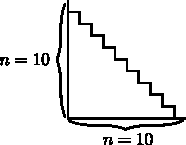
\includegraphics{staircase.pdf} 
\]
The upshot is that in essence, to lay a staircase of $n$ stairs that
is up to code in a space that is $w$ feet wide and $h$ feet tall, you
must solve the following equation:
\[
\mat{D}_{s,t}
\begin{bmatrix}
n \\
n \\
1
\end{bmatrix}
= 
\begin{bmatrix}
w \\
h \\
1
\end{bmatrix}
\]
where 
$t\le \frac{31}{48}$ and $s\ge \frac{5}{6}$.

\begin{problem}
Where do the numbers 
\[
\frac{31}{48}\qquad\text{and}\qquad \frac{5}{6}
\]
come from?
\end{problem}


\begin{problem}
Carefully draw an $(s,t)$-plane, with $s$ on the horizontal axis and $t$ on the vertical axis. 
\begin{enumerate}
\item Shade in the region  $t\le \frac{31}{48}$ and $s\ge \frac{5}{6}$.
\item Expand the left-hand side of the following equation: 
\[
\mat{D}_{s,t}
\begin{bmatrix}
n \\ n \\ 1
\end{bmatrix}
= 
\begin{bmatrix}
w \\
h \\
1
\end{bmatrix}
\]
\item Now you should be able to write two equations. In each case, solve for $n$ and set these two equations equal to each other. 
\item Solve for $t$. Now you should have a single equation $t= \dots$.
\item Now you can set values for $w$ and $h$. Set $w = 15$ and $h=11$. Plot your equation on the $(s,t)$-plane.
\item Interpret your graph.  What do the different regions of the graph mean for our staircase?
\end{enumerate}
\end{problem}


\begin{problem}\label{P:Stair}
Suppose you wish to build a staircase that is $15'$ wide and $11'$
tall. What should be the dimensions of each step? How many different
solutions can you find?
\end{problem}

\begin{problem}
Suppose you wish to build a staircase that is $15'$ wide and $10'$
tall. What should be the dimensions of each step? How many different
solutions can you find?
\end{problem}

\begin{problem}
Suppose you wish to build a staircase that is $16'$ wide and $10'$
tall. What should be the dimensions of each step? How many different
solutions can you find?
\end{problem}


\begin{problem}
Smart Sam says he doesn't need matrices to solve
Problem \ref{P:Stair}. Instead, he says:
\begin{quote}
First you take the height of the staircase, $11'$, and divide it by
$31/48'$ to get $18$. Now take $15'$ and divide by $18$ to get
$5/6'$. So you have $18$ steps that are $5/6'$ deep and $31/48'$ tall.
\end{quote}
His arithmetic seems a bit strange to me---what is he doing?  Is his
solution different from what we did above? Hint: There are at least
two errors in his solution, one that is minor and another that is
major.
\end{problem}

\end{document}
